%===================================================================================
% JORNADA CIENTÍFICA ESTUDIANTIL 2013 - MATCOM, UH
%===================================================================================
% Esta plantilla ha sido diseñada para ser usada en los artículos de la
% Jornada Científica Estudiantil, MatCom 2015.
%
% Por favor, siga las instrucciones de esta plantilla y rellene en las secciones
% correspondientes.
%
% NOTA: Necesitará el archivo 'jcematcom.sty' en la misma carpeta donde esté este
%       archivo para poder utilizar esta plantila.
%===================================================================================



%===================================================================================
% PREÁMBULO
%-----------------------------------------------------------------------------------
\documentclass[a4paper,12pt,twocolumn]{article}

%===================================================================================
% Paquetes
%-----------------------------------------------------------------------------------
\usepackage{amsmath}
\usepackage{amsfonts}
\usepackage{amssymb}
\usepackage{jcematcom}
\usepackage[utf8]{inputenc}
\usepackage{listings}
\usepackage[pdftex]{hyperref}
%-----------------------------------------------------------------------------------
% Configuración
%-----------------------------------------------------------------------------------
\hypersetup{colorlinks,%
	    citecolor=black,%
	    filecolor=black,%
	    linkcolor=black,%
	    urlcolor=blue}

%===================================================================================



%===================================================================================
% Presentacion
%-----------------------------------------------------------------------------------
% Título
%-----------------------------------------------------------------------------------
\title{Problema 1: Returning Home}

%-----------------------------------------------------------------------------------
% Autores
%-----------------------------------------------------------------------------------
\author{\\
\name Rodrigo García Gómez\email \href{mailto:rodrigo.garcia@estudiantes.matcom.uh.cu}{rodrigo.garcia@estudiantes.matcom.uh.cu}
}

%-----------------------------------------------------------------------------------
% Tutores
%-----------------------------------------------------------------------------------
\tutors{\\
Alfredo Somoza \emph{} \\
}

%-----------------------------------------------------------------------------------
% Headings
%-----------------------------------------------------------------------------------


%-----------------------------------------------------------------------------------
\ShortHeadings{}{Autores}
%===================================================================================



%===================================================================================
% DOCUMENTO
%-----------------------------------------------------------------------------------
\begin{document}

%-----------------------------------------------------------------------------------
% NO BORRAR ESTA LINEA!
%-----------------------------------------------------------------------------------

%-----------------------------------------------------------------------------------
\twocolumn[
\maketitle

%===================================================================================
% Resumen y Abstract
%-----------------------------------------------------------------------------------
\selectlanguage{spanish} % Para producir el documento en Español

%-----------------------------------------------------------------------------------
% Resumen en Español
%-----------------------------------------------------------------------------------
\begin{abstract}
Dado un tablero cuadrado de $n$ posiciones, se debe buscar la mejor forma de llegar de la posición inicial al destino, teniendo en cuenta la existencia de posiciones de desplazamiento instantáneo.
Primeramente se implementó un algoritmo de “fuerza bruta” que prueba todos los caminos posibles que se pueden recorrer desde la salida hasta el destino, teniendo en cuenta los saltos instantáneos, y realiza una comparación para obtener el de menos costo de tiempo. Este algoritmo tiene una complejidad temporal exponencial y es altamente ineficiente, lo que provocó dificultades en el proceso de testeo de la solución óptima a partir de la comparación. Debido a esto se hizo otro algoritmo de fuerza bruta, parecido al anterior, pero moderadamente optimizado. Finalmente se implementó un algoritmo óptimo, el cual forma un grafo que tiene como vértices la posición inicial y todos los puntos de desplazamiento instantáneo; la solución al problema es el mínimo entre las distancias de cada nodo con respecto a la posición inicial, sumadas con su distancia con respecto a la posición final.
\end{abstract}

%-----------------------------------------------------------------------------------
% English Abstract
%-----------------------------------------------------------------------------------
\vspace{0.5cm}



%-----------------------------------------------------------------------------------
% Palabras clave
%-----------------------------------------------------------------------------------


%-----------------------------------------------------------------------------------
% Temas
%-----------------------------------------------------------------------------------



%-----------------------------------------------------------------------------------
% NO BORRAR ESTAS LINEAS!
%-----------------------------------------------------------------------------------
\vspace{0.8cm}
]
%-----------------------------------------------------------------------------------


%===================================================================================

%===================================================================================
% Introducción
%-----------------------------------------------------------------------------------
\section{Texto del problema} 

	Yura has been walking for some time already and is planning to return home. He needs to get home as fast as possible. To do this, Yura can use the instant-movement locations around the city.\\
	Let's represent the city as an area of $n$x$n$ square blocks. Yura needs to move from the block with coordinates ($s_x$,$s_y$) to the block with coordinates ($f_x$,$f_y$). In one minute Yura can move to any neighboring by side block; in other words, he can move in four directions. Also, there are m instant-movement locations in the city. Their coordinates are known to you and Yura. Yura can move to an instant-movement location in no time if he is located in a block with the same coordinate x or with the same coordinate y as the location.\\
	Help Yura to find the smallest time needed to get home.

\section{El problema} 
   Se cuenta con un tablero cuadrado de $n\times n$ posiciones. Existen $m$ posiciones de movimiento instantáneo (moverse hacia ellas no tiene costo). Se debe encontrar la forma con menor costo de moverse de la posición de coordenadas $(s_x, s_y)$ a la de coordenadas $(f_x, f_y)$. Moverse hacia una posición adyacente tiene costo 1. Las posiciones de las localizaciones de movimiento instantáneo son conocidas y es posible moverse hacia ellas sin costo de tiempo si tienen igual coordenada $x$ o igual coordenada $y$ que la posición actual.
  

%===================================================================================



%===================================================================================
% Desarrollo
%-----------------------------------------------------------------------------------
\section{Algoritmo de Dijkstra}

 Se utiliza para hallar la distancia mínima entre un vértice $u$ y todos los vértices del grafo. Durante la ejecución del algoritmo se va actualizando una lista \texttt{\ttfamily distances }que al finalizar tendrá para la posición $v$ la distancia mínima entre $v$ y $u$. Todas las distancias inician con valor \texttt{\ttfamily sys.maxsize}, excepto por la del vértice inicial (que será $u$), pues claramente la distancia de $u$ a $u$ es 0. En cada iteración del ciclo principal se busca por el vértice $v$ que actualmente sea más cercano a $u$ y que todavía no haya sido visitado por el algoritmo (el primero será $u$ pues es el único con distancia menor que \texttt{\ttfamily sys.maxsize}). Teniendo a este vértice se analizarán todos sus adyacentes $k$ y, si el costo de la arista que une a $v$ con $k$ sumado con la distancia de $v$ a $u$ es menor que la distancia actual entre $u$ y $k$, entonces se actualiza la distancia de $u$ a $k$, dándole el valor de la distancia de u a v más el costo de la arista $<u, k>$. El ciclo se ejecutará mientras queden nodos por visitar y de estos el de menor valor en \texttt{\ttfamily distances} sea distinto de \texttt{\ttfamily sys.maxsize} pues, esto significa que sólo quedan nodos que no están conectados con $u$ (note que si no existe camino de $u$ a algún nodo $x$ entonces \texttt{\ttfamily distances[x] = sys.maxsize}).


	\subsection{Demostración}

		Se demostrará que al finalizar la ejecución de Dijkstra quedará en  \texttt{\ttfamily distances[i]} la distancia mínima entre $u$ y el nodo $i$. De no existir camino entonces \texttt{\ttfamily distances[i] = sys.maxsize}.
		
		Sea $V$ el conjunto de todos los vértices, $Vis$ el conjunto de los vértices que ya han sido visitados y $dis(u,v)$ el camino mínimo de $u$ a $v$. En cada iteración se cumple que:


		\begin{enumerate}
			\item Para cada $v$ que pertenece a $Vis$, cualquier camino de $u$ a $v$ tiene costo al menos  \texttt{\ttfamily distances[v]}
			\item Existe un camino de $u$ a $v$ con costo \texttt{\ttfamily distances[v]}
		\end{enumerate}
		\subsubsection{Inducción sobre las iteraciones ($it$) del ciclo principal}
		Para $$it = 0$$
		Se tiene que $Vis = \emptyset$. En la primera iteración se visita $u$, ya que es el único con distancia menor que \texttt{\ttfamily sys.maxsize} y por tanto $Vis$ = { $u$ }. El costo de u a u es 0 y existe el camino, que es vacío.\\
			
			$$it \Rightarrow it + 1$$\\
			
			Los únicos vértices que actualizan su valor en \texttt{\ttfamily distances} son aquellos que están conectados a alguno de los vértices ya visitados en iteraciones anteriores, por tanto, el vértice seleccionado para visitar en esta iteración ($v$) lo está, pues tendrá valor menor que \texttt{\ttfamily sys.maxsize}. Además, este tendrá como distancia a $$\texttt{\ttfamily distances[k]}  +  costo(<k, v>)$$ siendo $k$ el vértice que cumple que entre todos los vértices $k_0$ que pertenecen a $Vis$ y están conectados con $v$, es mínima la suma:
			 $$ \texttt{\ttfamily distances[$k_0$]} + costo(<k_0,v>)$$
			Esto significa que la mejor forma de llegar a $v$ por sus nodos adyacentes que pertenecen a $Vis$ es saliendo de k, pues es el que suma un menor costo.\\
			Note que no existe vértice $v_1$ que no pertenece a $Vis$, adyacente con $v$, tal que se pueda formar un camino de $u$ a $v$ pasando por $v_1$ con costo menor que $\texttt{\ttfamily distances[k]} + costo(<k, v>)$.	Esto se debe a que, de ser $v_1$ adyacente con alguno de los vértices de $Vis$, el solo costo de llegar a $v_1$ ya sería mayor o igual que el de llegar a $v$ directamente saliendo de un vértice de $Vis$ (peor aún si a esto se le suma $costo(<v_1, v>)$) y de $v_1$ no ser adyacente con ningún vértice de $Vis$, habría que pasar por uno que sí lo fuera para llegar a él, y el costo de llegar a este fuera también mayor o igual que el de llegar a $v$ directamente, pues $v$ es el más cercano a los vértices de $Vis$. ambos casos se ilustran en la Figura 1.\\
			\begin{figure} [h!]
				\centering
				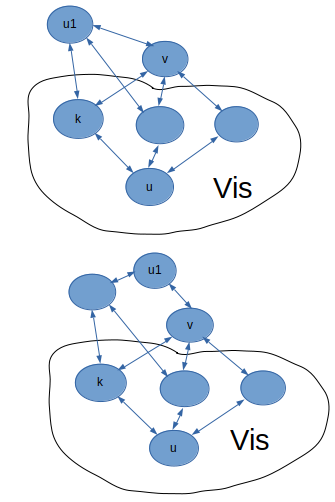
\includegraphics[width=0.8\linewidth]{figura1}
				\caption{Se ilustra cuando $u_1$ es adyacente a algún vértice de $Vis$ y cuando no lo es. En ambos casos es más costoso llegar a $v$ pasando por $u_1$ que partiendo desde $k$ pues $v$ es el más cercano a cualquier vértice perteneciente a $Vis$}
				\label{fig:figura1}
			\end{figure}
			
			Por hipótesis de inducción se tiene que la distancia de $u$ a $k$ almacenada en \texttt{\ttfamily distances[k]} es mínima y que hay una forma de llegar de $u$ a $k$ con este costo. Como ya se demostró que no existe mejor forma de llegar a $v$ que saliendo de $k$ y \texttt{\ttfamily distances[k]} es la mejor forma de llegar a $k$, $$\texttt{\ttfamily distances[k]} + costo(<k, v>)$$ es la mejor forma de llegar a $v$, y existirá forma de hacerlo, pues basta con formar un camino uniendo la forma de llegar a $k$ con ese costo y agregarle la arista $<k, v>$.\\
			
			Se ha demostrado que para todos los vértices que pertenezcan a $Vis$ al llegar a la última iteración, se habrá calculado la distancia mínima. Sólo aquellos que no son adyacentes a algún vértice que pertenezca a la misma componente conexa de $u$ no verán su valor en \texttt{\ttfamily distances} cambiado y al tratar de visitar el primero de estos vértices el algoritmo se detendrá, pues significará que no queda ningún 	vértice cuyo valor en \texttt{\ttfamily distances} ha sido modificado a un valor menor que \texttt{\ttfamily sys.maxsize}, ningún vértice adyacente a alguno de $Vis$ (en $Vis$ quedan todos los que pertenezcan a la misma componente conexa de $u$).
	\section{Idea Fuerza Bruta}
		Consiste en revisar todos los posibles caminos que comienzan en el punto de partida y acaban en el de llegada. Se crea un tablero de $n \times n$ casillas que representa la ciudad. Este tablero se inicializa en 0 y se van marcando con 1 las posiciones a medida que se visitan; de esta forma se evita caer en ciclo infinito regresando a caminar por lugares ya visitados .Siendo $<x, y>$ la posición actual, se revisa en las cuatro direcciones, calculando de forma recursiva cuál es el menor costo a partir de cada una de estas y se les suma 1 para representar el costo de caminar hacia ellas. Además se busca en las cuatro direcciones la existencia de puntos de desplazamiento instantáneo y por cada uno que se encuentre, se revisa de forma recursiva el menor costo a partir de él (de forma similar a las revisiones anteriores, pero sin adicionar 1, pues desplazarse hacia ellos no tiene costo). Teniendo todos estos valores revisados, se retorna el menor. En cada llamado recursivo se marca con 1 la posición actual en el tablero, representada por las entradas $x$ y $y$; antes del retorno se vuelve a marcar esta posición con 0. El caso base de la recursión es alcanzar la posición final, en cuyo caso se retorna 0.
		
		La demostración de correctitud de este algoritmo se sustenta en el hecho de que son analizados todos los posibles caminos, así que de existir una solución esta será encontrada y en cada llamado recursivo se retorna la de menor costo.
		
		Siendo n el tamaño de la ciudad ($n^2$ la cantidad de casillas) y m la cantidad de zonas de desplazamiento instantáneo, el algoritmo pertenece a $O(2(n-1)(4 + m) ^{ n^2} )$ ya que en cada posición se tiene a lo sumo $4 + m$ posibles movimientos y esto se revisará a lo sumo $n^2$ veces para revisar de esta forma el tablero completo. El $2(n-1)$ se debe a las revisiones que se hacen en cada ejecución de la función recursiva para buscar las posiciones instantáneas, a lo largo del eje $x$ y del eje $y$. Por tanto la complejidad finalmente será: $O( 2n ( 4 + m) ^{ n ^ 2})$

	\section{Optimización de la Fuerza Bruta}
		La idea y la implementación son extremadamente similares a las del algoritmo anterior. La diferencia consiste en eliminar el chequeo de algunos casos innecesarios que se revisan varias veces. En el algoritmo original, cada vez que se llamaba recursivamente a la función, se revisaba en todas las direcciones para localizar las posiciones instantáneas y se visitaban todas, pero evidentemente, al desplazarse por un eje, las posiciones instantáneas de dicho eje serán las mismas y no es necesario volverlas a calcular. Además, al desplazarse por un eje no será necesario volver a desplazarse a las posiciones instantáneas de ese eje revisadas en la iteración anterior, pues valor resultante tendrá el mismo costo en caso de haberse desplazado a una posición instantánea, o un costo superior en exactamente una unidad en caso de haberse desplazado de forma no instantánea.\\
		
		Para lograr esto se agregan dos parámetros opcionales a la función. Estos son dos listas que representarán las posiciones instantáneas de los ejes $x$ y $y$. Sólo se buscará las posiciones instantáneas de los ejes con valor \texttt{\ttfamily None} en estos parámetros. Al desplazarse a una posición por un eje (ya sea desplazamiento instantáneo o no) se pasa a la función la lista de ese eje como una lista vacía, para indicar que ya no es necesario revisar las posiciones instantáneas de ese eje. La lista del otro eje se deja con valor por defecto (\texttt{\ttfamily None}) para recalcular las posiciones instantáneas.\\
	
		Estas podas hechas al algoritmo ayudan a que el proceso de testeo del siguiente algoritmo a partir de su comparación con la fuerza bruta sea más eficiente y abren la posibilidad de probar casos de mayor tamaño.
	
	\section{Algoritmo óptimo}

		De forma general, la idea consiste en armar un grafo que tiene como vértices a la posición inicial y a las posiciones de desplazamiento instantáneo. Los vértices estarán unidos por aristas que almacenarán la distancia que hay entre las posiciones en el mapa de los vértices. Sean $v$ y $u$ dos nodos, es posible desplazarse de forma instantánea desde $v$ hasta $u$ si tienen la misma coordenada $x$ o la misma coordenada $y$; esto indica que la arista $<v, u> = 0$. Por tanto la distancia entre dos nodos $v$, $u$ y el valor de la arista que los conecta estará dada por la menor de las diferencias entre sus coordenadas $x$ y sus coordenadas $y$ ($min( |x_v – x_u|, |y_v – y_u|)$). Esto se debe a que para llegar de $v$ a $u$ basta con alcanzar desde $v$ una coordenada $x$ o $y$ igual a alguna de $u$ (Figura 2).\\
		
		\begin{figure}[h!]
			\centering
			\includegraphics[width=0.9\linewidth]{"figura 2"}
			\caption{El valor de $<u,v>$ será 2, pues se llega a $a$ y se desplaza de forma instantánea}
			\label{fig:figura-2}
		\end{figure}
		
		Note que al tener dos nodos, $v$ y $u$, cuya distancia es $d = |x_v – x_u|$ (esto indica que son más cercanos por el eje $x$ que por el eje $y$. La demostración para el caso inverso es análoga), de tener un vértice $k$, cuya coordenada $x_k$ está entre $x_v$ y $x_u$ $(min(x_v,x_u) <= x_k <= max(x_v, x_u))$ entonces la distancia entre $u$ y $v$ será igual a la distancia entre $v$ y $k$ más la distancia entre $k$ y $u$. Esto se debe a que, suponiendo sin pérdida de generalidad que $x_v > x_u$, entonces\\
		
			$$d(v, u) = x_v – x_u$$
		como    $$x_u <= x_k <= x_v$$\\
		entonces  $$d(v, k) = x_v – x_k$$
		y 	    $$d(u, k) = x_k – x_u$$\\
		$$\Rightarrow d(v, k) + d(k, u) = x_v – x_k + x_k – x_u = x_v – x_u $$\\
		$$\Rightarrow  d(v, k) + d(k, u) = d(v, u)$$\\
		
		Todo esto indica que la arista $<v, u>$ es innecesaria y puede ser removida del grafo.\\
		
		*(en este caso $d(v, k)$ y $d(u, k)$ son las distancias con respecto al eje $x$ y no las distancias finales de las aristas, pues $k$ puede estar más cerca por el eje $y$ a $v$ o a $u$. De ser este el caso, las distancias serían menores, por lo que de cualquier forma, la arista $e(v, u)$ sobraría)\\
		
		Basándose en lo anterior queda claro que, dado un vértice v, sólo necesita estar enlazado con, los vértices $u_1$, $u_2$, $u_3$ y $u_4$ que cumplan lo siguiente:
		\begin{enumerate}
		\item 	$u_{1x} > x_v$ y no puede existir un $k$ tal que $u_{1x} > x_k > x_v$
		\item $u_{1x} > x_v$ y no puede existir un $k$ tal que $u_{1x} > x_k > x_v$
		\item $u_{2x} < x_v $y no puede existir un k tal que $u_{1x} < x_k < x_v$
		\item $u_{3y} > y_v$ y no puede existir un $k$ tal que ${u_{1y}} > y_k > y_v$
		\item $u_{4y} < y_v$ y no puede existir un $k$ tal que $u_{1y} < y_k < y_v$
		\end{enumerate}
		*(note que pueden haber más de un nodo que cumpla con una de estas propiedades, en ese caso el algoritmo sólo deja la arista con uno y garantiza que los otros estén conectados entre sí)\\
		*(note además que $u_1$, $u_2$, $u_3$ o $u_4$ pueden no existir o ser todos el mismo nodo)\\
		Todo esto significa que el vértice $v$ estará enlazado con los vértices más cercanos hacia cada una de las cuatro direcciones.\\
			
		Una vez se tiene formado dicho grafo ($G$), se aplica sobre él el algoritmo de Dijkstra para calcular la distancia del menor camino de cada nodo hacia el nodo inicial ($s$). Luego a cada una de esas distancias se le suma la distancia desde su nodo hasta el nodo final, calculada como $| x_v - x_f| + | y_v – y_f|$ y se retorna el menor valor entre todas estas distancias.\\
		
		Demostrando que la solución encontrada es la mejor posible\\
		Suponga que se tiene un camino $c_1$ cuyo costo es menor que el camino hayado $c$, $s$ y $f$ son los nodos iniciales y finales respectivamente. Además \texttt{\ttfamily d} es el arreglo que tiene las distancias halladas por el algoritmo, de las cuales se escogió para retornar el valor mínimo. Si $c_1$ no pasara por ninguna posición de desplazamiento instantáneo, entonces $c_1$ tiene que ser mayor o igual que el valor en la primera posición de \texttt{\ttfamily d}, ya que este posee la distancia de caminar directamente de $s$ a $f$con pasos de un minuto.\\
		Entonces $c_1$, para tener costo menor que \texttt{\ttfamily d[0]} debe pasar por al menos una de las posiciones de desplazamiento instantáneo. Sea $t$ el último de estos desplazamientos por los que pasa $c_1$ antes de ir directo a $f$, existe un valor $d_i$ de \texttt{\ttfamily d} que representa el valor del menor camino en $G$, desde el nodo $s$ hasta el nodo $t$, sumando con la distancia de $t$ a $f$. La distancia desde $t$ a $f$ de $c_1$ debe ser mayor o igual que la distancia desde $t$ a $f$ de $d_i$, porque este posee la distancia de caminar directamente hacia $f$ con pasos de un minuto. Además, la distancia de $s$ a $t$ representada por $d_i$ es la menor posible, siendo esto garantizado por el algoritmo de Dijkstra realizado sobre el grafo $G$ (que por la forma en que fue construido contempla, o contempló en algún momento y eliminó por innecesaria, cada una de las formas de ir de la salida a cualquier punto instantáneo, ya sea yendo directamente o pasando por otros puntos instantáneos). Por tanto, la distancia de $s$ a $t$ en $c_1$ debe ser mayor o igual que la distancia de $s$ a $t$ representada por $d_i$. Luego el costo de tiempo de $c_1$ debe ser mayor o igual que $d_i$.\\
		Como el costo de $c_1$ debe ser mayor o igual que alguno de los valores de $d$, y $c$ es el menor de estos valores, el costo $c_1$ debe ser mayor o igual que $c$, lo que implica que no existe camino $c_1$ con costo menor que el costo $c$ devuelto por el algoritmo.
		\subsection{Complejidad temporal}
			Hay cuatro ciclos de $m$ iteraciones ($O(m)$), dos ordenaciones ($O(n  log n)$), y una ejecución de Dijkstra, que como $m$ es igual a la cantidad de vértices de $G$ y siendo $E$ la cantidad de aristas (puede ser a lo sumo $\frac{m(m-1)}{2})$ pertenece a $O(E + m log m)$, como $m<=n$, entonces el costo del algoritmo pertenece a $O(E + n log n)$.
%-----------------------------------------------------------------------------------
\label{end}

\end{document}

%===================================================================================
